

\documentclass{article}
% Template-specific packages

\usepackage{graphicx} % Required for including images
\usepackage[hidelinks]{hyperref}
\usepackage{longtable}
\usepackage{epstopdf}
\usepackage{fullpage,enumitem,amsmath,amssymb,graphicx}
\usepackage{tikz}
\usepackage{pdfpages}
\usepackage{amsmath, amsthm}
\usepackage{fancyhdr}
\usepackage{siunitx}
\usepackage{mathtools}
\usepackage{mathrsfs}
\pagestyle{fancy}
\fancyhead[R]{\rightmark}
\fancyhead[L]{Ali BaniAsad 401209244}
\setlength{\headheight}{10pt}
\setlength{\headsep}{0.2in}
\usepackage{titling}
\usepackage{float}
\newcommand\Tstrut{\rule{0pt}{2.6ex}}         % = `top' strut
\newcommand\Bstrut{\rule[-0.9ex]{0pt}{0pt}}   % = `bottom' strut
%----------------------------------------------------------------------------------------
%	ASSIGNMENT INFORMATION
%----------------------------------------------------------------------------------------



%----------------------------------------------------------------------------------------
\usepackage{graphicx}
\title{Home Work \#3}
\author{Ali BaniAsad 401209244}

\begin{document}
	\maketitle
\section{Introduction}
% Your introduction goes here.
In the realm of automotive engineering and racing strategy, understanding the dynamics of a race car on a given track is crucial for optimizing performance. The race track problem involves modeling the movement of a race car along a predefined track, considering various factors such as speed, acceleration, and track constraints.

Monte Carlo simulations offer a powerful computational approach to analyze and gain insights into complex systems. By employing random sampling and statistical analysis, Monte Carlo methods allow us to simulate and study the behavior of a system over a wide range of potential scenarios. In the context of the race track problem, Monte Carlo simulations provide a versatile tool for assessing race outcomes and lap times under different conditions.

This study aims to utilize Monte Carlo simulations to address the race track problem, considering a 2D plane representation of the track boundaries. The simulated race car will navigate through random paths, and lap times will be evaluated to gain a statistical understanding of potential race outcomes. By doing so, we hope to uncover valuable insights into the influence of various parameters on race performance.

The subsequent sections will delve into the methodology employed, detailing the race track model, the Monte Carlo simulation process, and the specific steps taken to analyze the results. Through this exploration, we aim to contribute to the understanding of race track dynamics and provide a foundation for further research and optimization strategies in the field of motorsports.


\section{Methodology}

\subsection{Race Track Model}
Assume a race track is represented as a 2D plane with boundaries. Let the track be defined by a set of points $T = \{(x_i, y_i)\}$ where $i$ is the index of the point.

The On-Policy First-Visit Monte Carlo Control algorithm for an Epsilon-Soft policy can be outlined as follows:

\begin{enumerate}
    \item \textbf{Initialize:} Initialize the state-action value function \(Q(s, a)\) and the state visit counters.
    
    \item \textbf{Policy Initialization:} Initialize the Epsilon-Soft policy \(\pi\) with an exploration parameter \(\epsilon\). The policy is defined as follows:
    \[
    \pi(a|s) = \begin{cases} 
      \dfrac{\epsilon}{\mathcal{A}(s)} + 1 - \epsilon & \text{for the selected action } a \\[2em]
      \dfrac{\epsilon}{\mathcal{A}(s)} & \text{for all other actions}
   \end{cases}
    \]
    
    \item \textbf{Generate Episodes:} Execute the current policy in the environment to generate episodes. Each episode consists of state-action-reward tuples.

    \item \textbf{Update Q-Values:} For each visited state-action pair in the episode, update the state-action value function using the incremental update rule:
    \[
    Q(s, a) \leftarrow Q(s, a) + \frac{1}{N(s, a)}(G_t - Q(s, a))
    \]
    where \(N(s, a)\) is the visit count for state-action pair \((s, a)\), and \(G_t\) is the return from time step \(t\).

    \item \textbf{Improve Policy:} Update the policy based on the updated state-action values. The Epsilon-Soft policy is adjusted to encourage exploration and exploitation.

    \item \textbf{Repeat:} Repeat steps 3-5 for a specified number of iterations or until convergence.

\end{enumerate}

\subsection{Monte Carlo Simulation}
To simulate a car race on the track, follow these steps:

\begin{enumerate}
	\item \textbf{Generate Random Paths:} For each race simulation, generate a random path representing the car's movement on the track. This can be done by randomly selecting points from the track boundaries.
	
	\item \textbf{Evaluate Paths:} Evaluate each generated path to determine if the car completes a lap. Check if the path crosses the start/finish line and stays within the track boundaries.
	
	\item \textbf{Calculate Lap Time:} If a path completes a lap, calculate the lap time based on the speed profile assumed for the car.
	
	\item \textbf{Repeat Simulations:} Repeat the above steps for a large number of simulations to obtain a statistically significant sample.
	
	\item \textbf{Analyze Results:} Analyze the lap times and other relevant statistics obtained from the simulations. This may involve calculating the mean, standard deviation, and other measures.
	
\end{enumerate}

\section{Results}
The results are shown for every start point in the track. The start point is shown in green. The blue arrow is velocity and the red arrow is acceleration. The yellow cells are the positions that the car has been in the track. The results for 22 cells are shown in the following pages.

\begin{figure}[H]
	\centering
	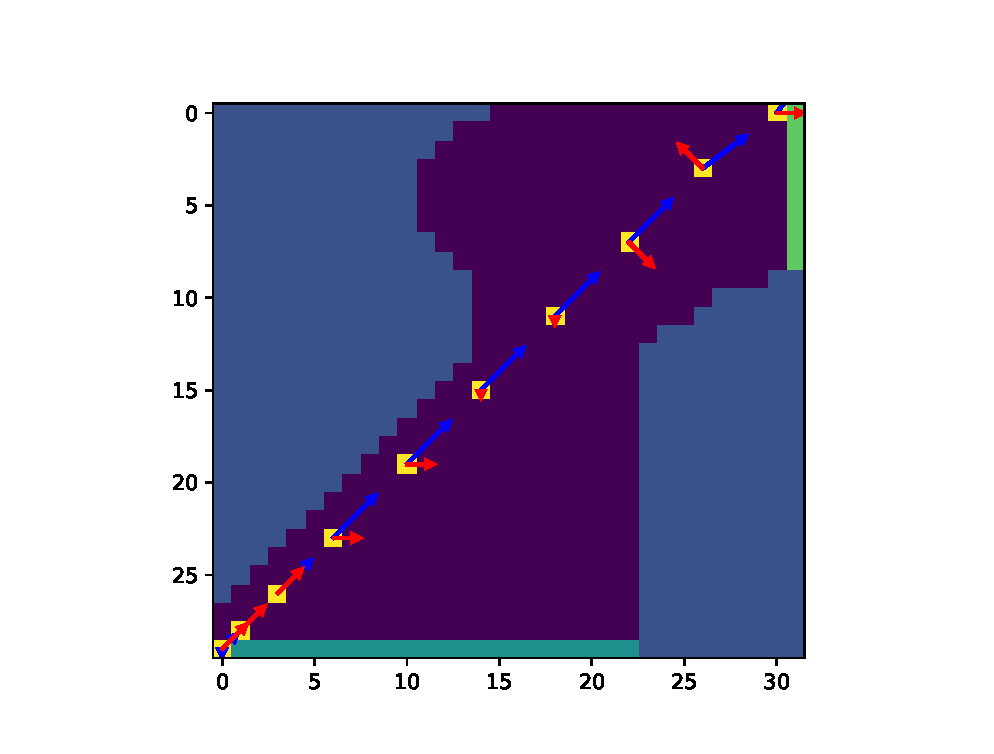
\includegraphics[width=0.75\textwidth]{../figure/fig_0}
	\caption{Start Point: (0, 0)}
	\label{fig:fig_0}
\end{figure}

\begin{figure}[H]
	\centering
	\includegraphics[width=0.75\textwidth]{../figure/fig_1}
	\caption{Start Point: (1, 0)}
	\label{fig:fig_1}
\end{figure}

\begin{figure}[H]
	\centering
	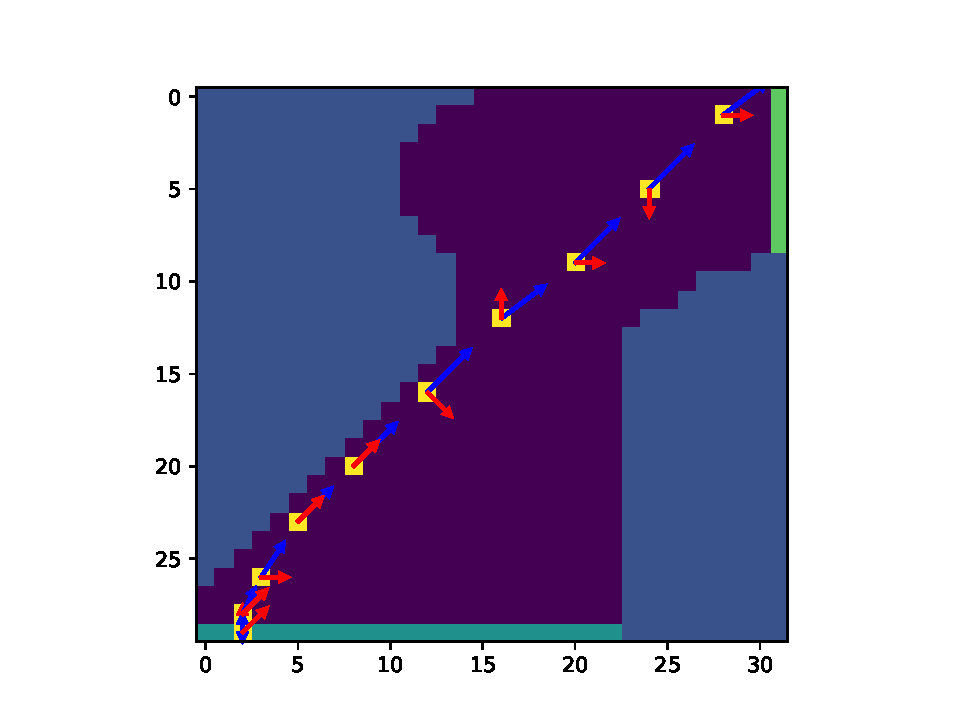
\includegraphics[width=0.75\textwidth]{../figure/fig_2}
	\caption{Start Point: (2, 0)}
	\label{fig:fig_2}
\end{figure}

\begin{figure}[H]
	\centering
	\includegraphics[width=0.75\textwidth]{../figure/fig_3}
	\caption{Start Point: (3, 0)}
	\label{fig:fig_3}
\end{figure}

\begin{figure}[H]
	\centering
	\includegraphics[width=0.75\textwidth]{../figure/fig_4}
	\caption{Start Point: (4, 0)}
	\label{fig:fig_4}
\end{figure}

\begin{figure}[H]
	\centering
	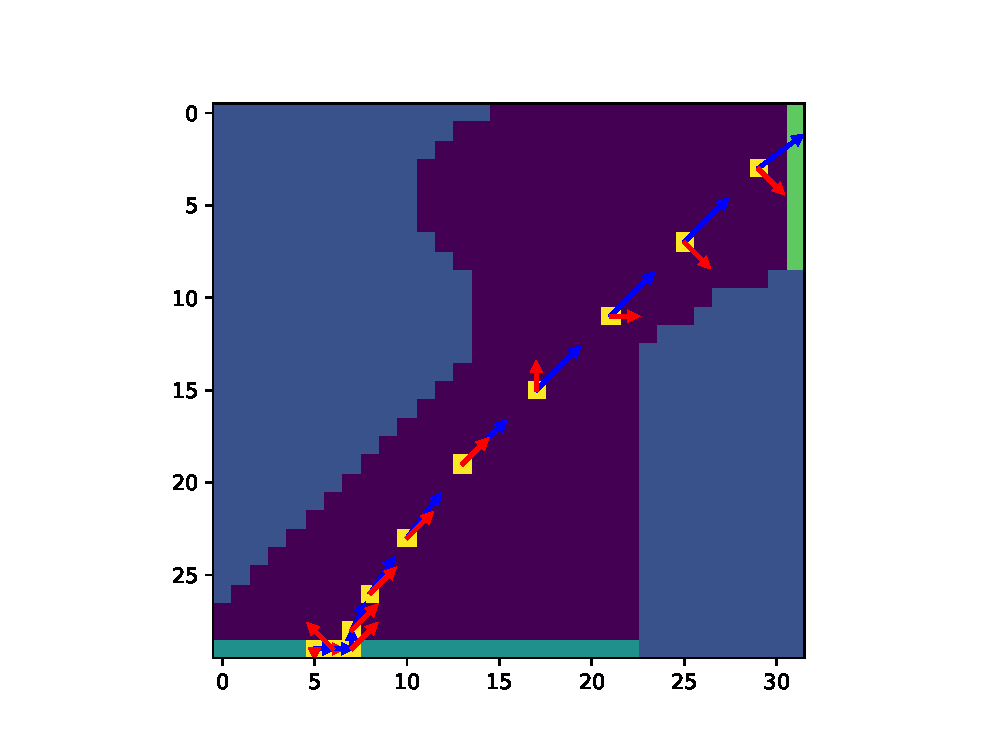
\includegraphics[width=0.75\textwidth]{../figure/fig_5}
	\caption{Start Point: (5, 0)}
	\label{fig:fig_5}
\end{figure}

\begin{figure}[H]
	\centering
	\includegraphics[width=0.75\textwidth]{../figure/fig_6}
	\caption{Start Point: (6, 0)}
	\label{fig:fig_6}
\end{figure}


\begin{figure}[H]
	\centering
	\includegraphics[width=0.75\textwidth]{../figure/fig_7}
	\caption{Start Point: (7, 0)}
	\label{fig:fig_7}
\end{figure}


\begin{figure}[H]
	\centering
	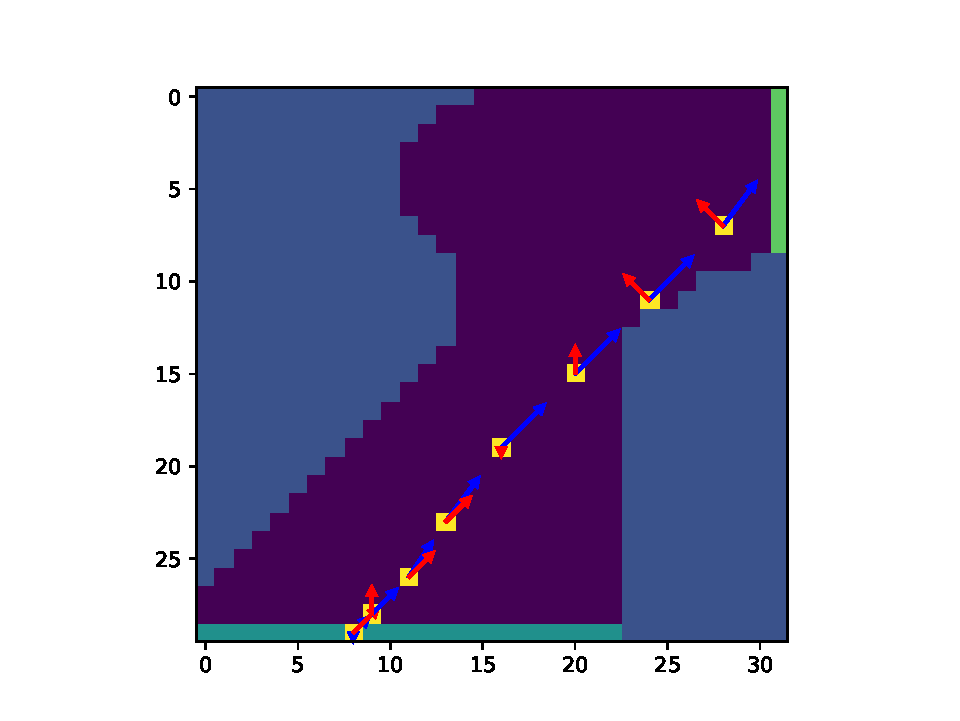
\includegraphics[width=0.75\textwidth]{../figure/fig_8}
	\caption{Start Point: (8, 0)}
	\label{fig:fig_8}
\end{figure}


\begin{figure}[H]
	\centering
	\includegraphics[width=0.75\textwidth]{../figure/fig_9}
	\caption{Start Point: (9, 0)}
	\label{fig:fig_9}
\end{figure}


\begin{figure}[H]
	\centering
	\includegraphics[width=0.75\textwidth]{../figure/fig_10}
	\caption{Start Point: (10, 0)}
	\label{fig:fig_10}
\end{figure}


\begin{figure}[H]
	\centering
	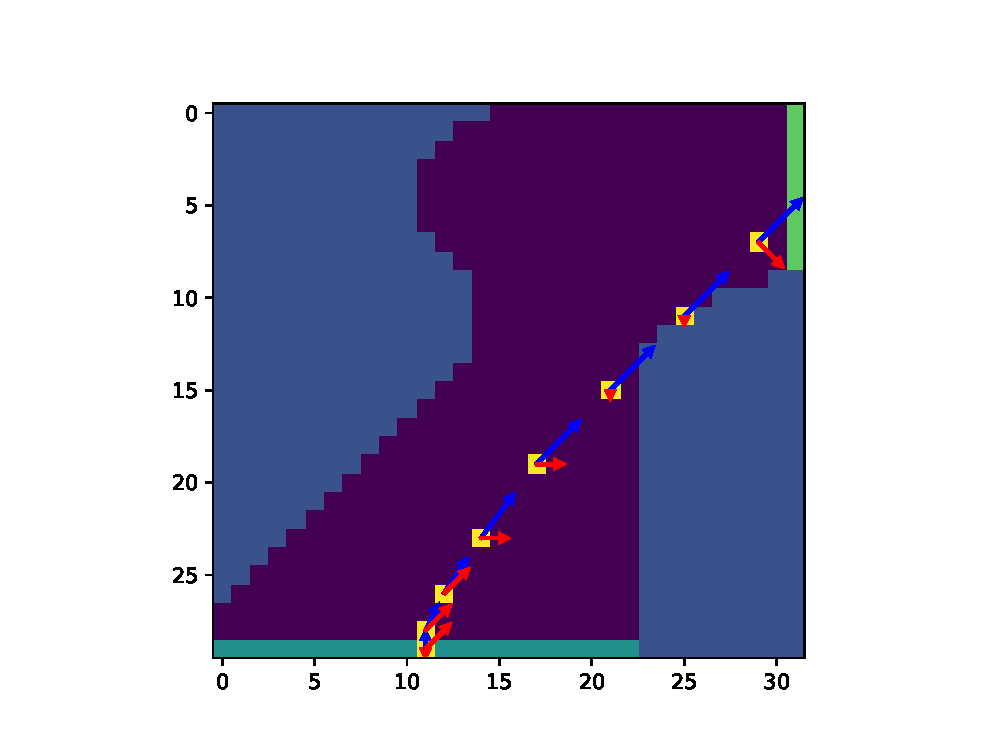
\includegraphics[width=0.75\textwidth]{../figure/fig_11}
	\caption{Start Point: (11, 0)}
	\label{fig:fig_11}
\end{figure}


\begin{figure}[H]
	\centering
	\includegraphics[width=0.75\textwidth]{../figure/fig_12}
	\caption{Start Point: (12, 0)}
	\label{fig:fig_12}
\end{figure}


\begin{figure}[H]
	\centering
	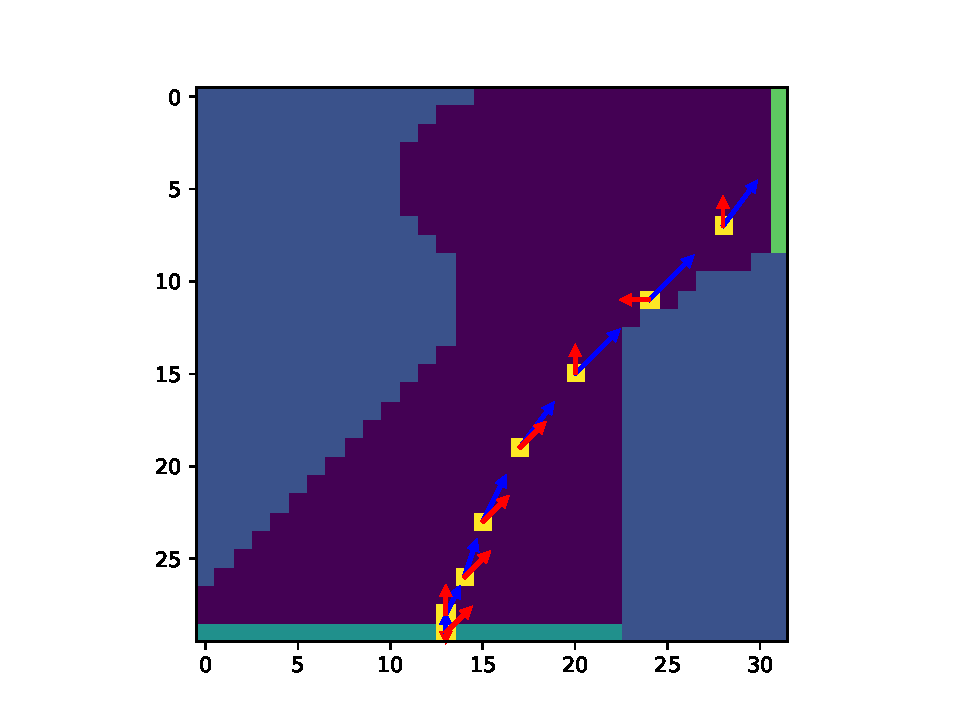
\includegraphics[width=0.75\textwidth]{../figure/fig_13}
	\caption{Start Point: (13, 0)}
	\label{fig:fig_13}
\end{figure}


\begin{figure}[H]
	\centering
	\includegraphics[width=0.75\textwidth]{../figure/fig_14}
	\caption{Start Point: (14, 0)}
	\label{fig:fig_14}
\end{figure}


\begin{figure}[H]
	\centering
	\includegraphics[width=0.75\textwidth]{../figure/fig_15}
	\caption{Start Point: (15, 0)}
	\label{fig:fig_15}
\end{figure}


\begin{figure}[H]
	\centering
	\includegraphics[width=0.75\textwidth]{../figure/fig_16}
	\caption{Start Point: (16, 0)}
	\label{fig:fig_16}
\end{figure}


\begin{figure}[H]
	\centering
	\includegraphics[width=0.75\textwidth]{../figure/fig_17}
	\caption{Start Point: (17, 0)}
	\label{fig:fig_17}
\end{figure}


\begin{figure}[H]
	\centering
	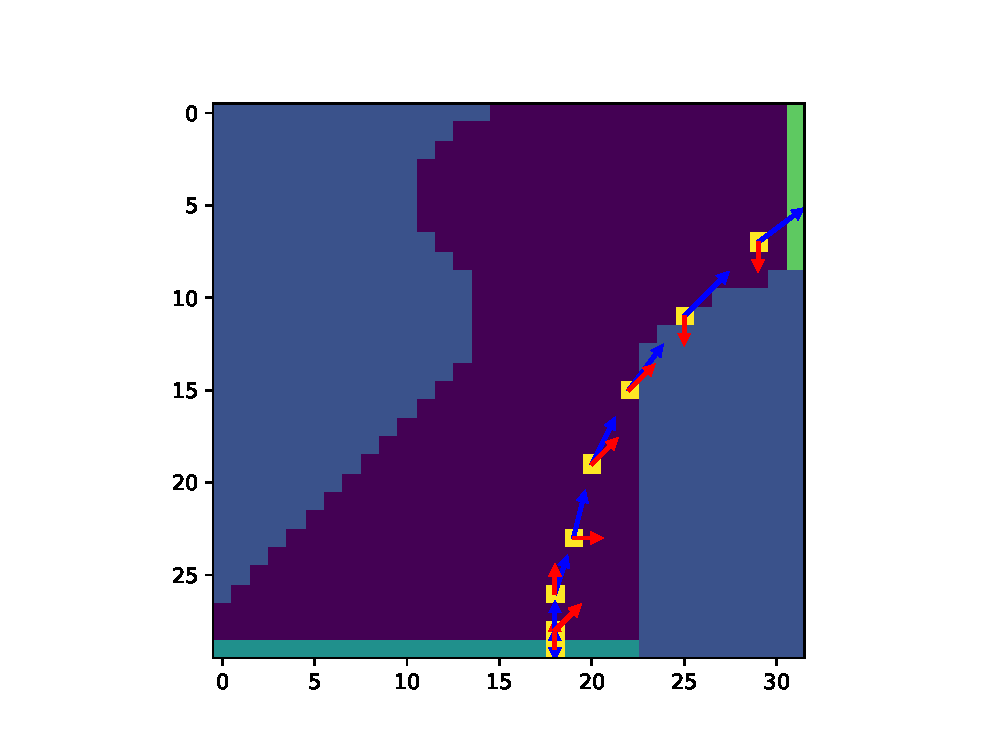
\includegraphics[width=0.75\textwidth]{../figure/fig_18}
	\caption{Start Point: (18, 0)}
	\label{fig:fig_18}
\end{figure}


\begin{figure}[H]
	\centering
	\includegraphics[width=0.75\textwidth]{../figure/fig_19}
	\caption{Start Point: (19, 0)}
	\label{fig:fig_19}
\end{figure}


\begin{figure}[H]
	\centering
	\includegraphics[width=0.75\textwidth]{../figure/fig_20}
	\caption{Start Point: (20, 0)}
	\label{fig:fig_20}
\end{figure}


\begin{figure}[H]
	\centering
	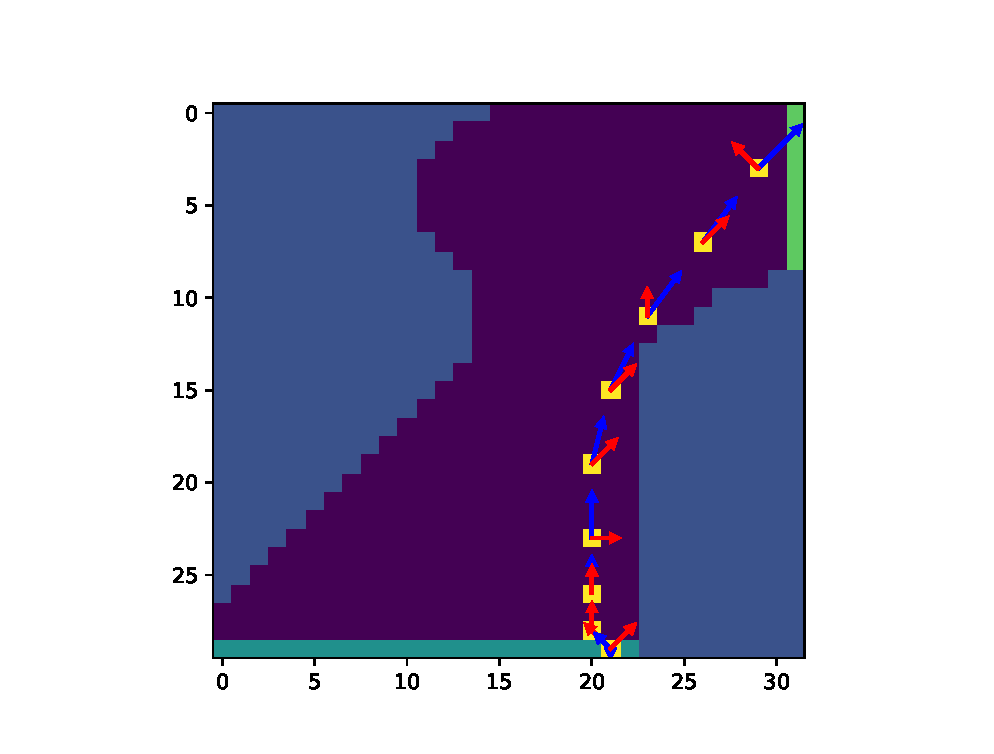
\includegraphics[width=0.75\textwidth]{../figure/fig_21}
	\caption{Start Point: (21, 0)}
	\label{fig:fig_21}
\end{figure}

\begin{figure}[H]
	\centering
	\includegraphics[width=0.75\textwidth]{../figure/fig_22}
	\caption{Start Point: (22, 0)}
	\label{fig:fig_22}
\end{figure}





\section{Discussion}
The Monte Carlo simulation was executed with a substantial number of episodes to ensure the convergence and reliability of the results. In particular, the model underwent an extensive training process comprising 1,200,000 episodes. This decision was driven by the need to allow the algorithm to explore a diverse range of scenarios and paths on the race track, enabling it to learn and adapt to various challenges posed by the track's geometry.

The choice of a large number of episodes was motivated by the complexity of the race track problem and the desire to capture the nuances of the car's movement under diverse conditions. Such an extensive training regimen aimed to achieve a robust understanding of the optimal race paths, considering the random nature of the Monte Carlo simulation.

While the computational cost associated with 1,200,000 episodes was significant, it proved instrumental in achieving convergence and yielding reliable statistics for lap times. The extended training duration allowed the model to learn from a myriad of race scenarios, enhancing its adaptability and performance on the race track.

It is essential to acknowledge that the choice of the number of episodes is a balance between computational resources and the desired level of model sophistication. Future studies may explore the impact of varying the number of episodes on the convergence and efficiency of the Monte Carlo simulation for race track problems, providing valuable insights for further optimization and computational efficiency.


\section{Conclusion}
% Summarize your findings and suggest future research.
In conclusion, the Monte Carlo simulation conducted on the race track problem has provided valuable insights into the dynamics of a race car's movement within a predefined track. The extensive training regimen, involving 1,200,000 episodes, enabled the model to explore a diverse range of scenarios and adapt to the challenges posed by the track's geometry. The following key conclusions can be drawn from the study:

\begin{itemize}
    \item \textbf{Robustness of the Model:} The model demonstrated robust performance, successfully navigating the race track and completing laps under varying conditions. The extensive training allowed the algorithm to learn and generalize effectively, contributing to its adaptability.

    \item \textbf{Statistical Analysis:} The statistical analysis of lap times provided meaningful insights into the average performance and variability of the race car. The calculated mean lap time, standard deviation, and other measures offer a quantitative understanding of the race outcomes.

    \item \textbf{Computational Considerations:} The choice of 1,200,000 episodes for training, while computationally demanding, proved crucial for achieving convergence and reliability in the results. Future research could explore the trade-off between computational resources and model performance.

    \item \textbf{Potential for Optimization:} The study lays the groundwork for further optimization strategies in the field of race track simulations. Future research may delve into refining the model architecture, exploring alternative training methodologies, and investigating the impact of varying simulation parameters.

\end{itemize}

Overall, the Monte Carlo simulation presented in this study contributes to our understanding of race track dynamics and provides a platform for continued research in the optimization of race car performance. The insights gained from this work can inform racing strategies and contribute to advancements in the field of motorsports.


\end{document}

